\documentclass[10pt,twocolumn]{article}

% use the oxycomps style file
\usepackage{oxycomps}
\usepackage{comment}
\usepackage{graphicx}
\usepackage[toc,page]{appendix}



% usage: \fixme[comments describing issue]{text to be fixed}
% define \fixme as not doing anything special
\newcommand{\fixme}[2][]{#2}
% overwrite it so it shows up as red
\renewcommand{\fixme}[2][]{\textcolor{red}{#2}}
% overwrite it again so related text shows as footnotes
%\renewcommand{\fixme}[2][]{\textcolor{red}{#2\footnote{#1}}}

% read references.bib for the bibtex data
\bibliography{references}

% include metadata in the generated pdf file
\pdfinfo{
    /Title (PulseKeys: A Piano-Playing Rhythm Game)
    /Author (Compton French)
}

% set the title and author information
\title{PulseKeys: A Piano-Playing Rhythm Game}
\author{Compton French}
\affiliation{Occidental College}
\email{cfrench2@oxy.edu}

\begin{document}

\maketitle

\section{Introduction}

Many applications claim to teach people how to play an instrument. Applications such as \textit{Yousician}, \textit{Rocksmith+} and \textit{PianoVision} attempt to teach users to play piano across various mediums. \textit{Yousician} takes it users through a series of lessons as well as teaching versions of popular songs along the way. \textit{Rocksmith+} gives the user a range of songs within their catalog to play along with to their gamified interpretation. \textit{PianoVision} takes advantage of the Meta Quest's capabilities by allowing users to see the notes falling on to the piano keys in mixed reality. All of these products and more claim that users will 'learn' piano, but ultimately tread on the border of game experience and music education and failing to commit to one purpose. 

Rhythm games is a popular genre of video games that challenges players sense of rhythm by requiring them to respond to a song's rhythm, movements, and melodies. Various games in the genre gamify and emulate real world musical activites such as dancing with \textit{Dance Dance Revolution} and \textit{Dancerush Stardom}, playing a taiko drum with \textit{Taiko no Tatsujin}, playing various instruments in a band with \textit{Rock Band}, among others. There are also popular rhythm games whose gameplay does not mimic real instruments or activities associated with music such as clicking circles with \textit{Osu} and the platformer \textit{Geometry Dash}. The main similarity of these games is that they apply game design principles to keep player retention rates up, even if it does not translate directly to a practical life skill. I argue that piano applications such as \textit{Yousician}, \textit{Rocksmith+} and \textit{PianoVision} would be more successful by leaning into game design principles to make a game feel more fun and compete in a rhythm game environment. I support my argument by building a piano game prototype and surveying playtesters that demonstrates that users would play a gamified version of piano applications.


\section{Problem Context}
Music learning software such as \textit{Yousician}, \textit{Rocksmith+} and \textit{PianoVision} has the potential to be very helpful, but has problems from still being a high expense for people starting to learn, lack of motivation to practice outside of the application, and suboptimal teaching. However, by applications focusing on being a game, it can be an external source for autonomous motivation as an extension to proper music education.

\subsection{Expenses}
Applications geared towards people learning piano, have a price tag based on a monthly subscription model. More well-known applications are priced around \$10 a month to as high as \$90 a month \cite{SkoovePianoApps}. Previous game franchise \textit{Rocksmith} has their more gamified version of interactive music learning, \textit{Rocksmith+}, that is \$20 a month \cite{Rocksmith+}. Additionally, when it comes to some of the cheaper applications, there are other monetary gates. To play or practice with some of the applications, users will either need a piano or a compatible MIDI controller, which are not accessible to some groups of people. Mixed reality methods add another layer of fees in the fact that not everyone has access to a VR headset during the time of writing this paper. The potential has been demonstrated that the entry to learning music can be lowered, but all of these expenses only lowers the gate from traditional music lessons and not to the same level as buying and playing a video game. Creating my own open-source prototype allows for an even cheaper way to interact with the piano. 

\subsection{Lack of Motivation}
A major roadblock in people deciding to practice music on their own is because of a lack of motivation. People that are engaging with piano education software are attempting to supplement for cheaper and more accessible music education. Formal music education adopts a prescriptive, teacher-centered approach, limiting opportunities for self-regulated and intrinsically motivated learning which neglects creativity and enjoyment \cite{MotivationAndSelf-RegulationinMusicLearning}. People that do not find their own creativity and enjoyment in the software, will not find the motivation to continue. Further research emphasizes that autonomous motivation correlates with more frequent and higher-quality practice \cite{Self-DeterminedMotivationforPractice}. Music pedagogy recognizes the importance of self motivation and freedom in practicing music. 

However with video games, people do not work up motivation the same way as learning an educational subject and are usually a form of entertainment during downtime because it is fun. The video game industry, valued at \$183.9 billion in 2023, is a huge market that music software can tap into by applying game design principles to fit inside the rhythm games genre \cite{GamingRevenue}. In contrast to the existing piano applications previously listed, an accessible option to a video game based on a real instrument will reach a broader audience, and the gamified aspects will cause users to keep returning to the game. Games also help people achieve flow state and it is believed that music games can achieve the same result \cite{Wagner}. Previous success behind franchises such as \textit{Guitar Hero}, \textit{Rock Band}, \textit{Rocksmith}, and current success of \textit{Fortnite Festival} proves that there is a market for people that wish to engage with gamified music. While a piano game will not directly teach users how to play correctly, it can be a vehicle of motivation and enjoyment for playing an instrument. 

\subsection{Suboptimal teaching practices}
Even though a gamified version of interacting with instruments has the potential to attract a larger audience, students and music teachers have many criticisms on software that teaches people how to play piano. Online learning piano presents struggles in teaching other aspects of piano besides hitting correct notes and timing such as dynamics, pedaling, and other technical skills \cite{PianoTeachingandthePandemic}. Teachers also report that their inability to provide hands-on guidance may affect skill acquisition\cite{E-LearningPiano}. Computer computer-assisted instruction on piano education can also produce an over-reliance on the technology which leads to superficial learning and difficulties in retaining and reproducing music without technological aids \cite{Computer-AssistedInstructionPianoEducation}. The various issues on technology being a sole educator results in superficial and incorrect learning. While I argue that a piano game should not substitute other correct music education formats, students and teachers openness to music technology shows that it can be an extension of their education experience \cite{PianoTeachingAndLearningConcerns}. 

\section{Technical Background}

The main requirements of this game is the communication of information between the songs MIDI file and the user playing the game. Communication between the MIDI controller and MIDI files is the most important aspect of the entire game becasue The product will not work if there is disconnect between the inputs a user makes and the song they are trying to learn. The second most important quality is creating a game environment where users are comfortable to read and play a song on a MIDI controller. Understanding user interface (UI) and user experience (UX) principles are important to give users a fluid and enjoyable game experience. Achieving flow state and enjoyability in the piano game \cite{Wagner} is key to creating an environment for autonomous motivation. 

\subsection{Communication between MIDI Controllers and MIDI Files}

To build a piano game that utilizes a Musical Instrument Digital Interface (MIDI) controller, the most important interaction is communicating the MIDI signals from the device with the computer. MIDI is the standard to connect devices that make and control sound \cite{MIDIStandard}. Each input from a MIDI controller outputs an array of information to the computer, but the most important information for the project is the velocity (how hard a key is pressed), note down time, note up time, and pitch information. Velocity is communicated with a value between 0 and 127, where 0 is interpreted as note off and any value greater than 0 is intensity of the note played with 1 being the softest and 127 being the strongest. Note down and note up time communicates the intervals from inputs being pressed with ticks to measure time. Pitch information is also outputted as value from 0 to 127 where each number is a different note which is mapped to each key on a piano. Each input on the MIDI controller has to be accounted for accurately to preserve the importance of timing when playing music or a rhythm game. Additionally, MIDI inputs do not directly output audio, but it is the information that is communicated with the computer that allowed for audio to be processed. 

The game uses MIDI files to create the levels for each song. MIDI files stores one or more MIDI streams, with time information for each event. The MIDI files used in the game contains the information for each event including pitch and timing to play a song. The game parses through the pitch and note timing information in the file to determine the visual cues of notes falling onto the piano and the timings of inputs requested of the player.

\subsection{Game Environment and Rhythm Games}

The prototype presented in the paper is built using the Unity game engine. Other game engines were considered such as Unreal Engine 5, but was dropped because of the paywall for MIDI support and visualization. Unreal Engine 5 provided native MIDI device support into the engine at a base level, but had very expensive plug-ins for what I would need to incorporate through visualizations and parsing MIDI files \cite{MidiEngine3}. Unity does not have direct MIDI support, but the community around Unity has developed free ways to incorporate MIDI support. Imported support from \textit{DryWetMIDI}, and Keijiro's \textit{Minis} and \textit{MidiJack} provided the necessary support to build the prototype in the Unity environment. 

The prototype falls under a category of video games called rhythm games. Rhythm games is a genre of video games that focuses around players interacting with music while playing. Core components of rhythm games is the timing-based interactions and real-time feedback. A rhythm game that does not correctly sync the visual cues, audio, and correct timings together creates a horrible game experience. Users also receive real-time feed back for correct or incorrect inputs with visual and/or audio signifiers. Gathering playtesters across various experience levels and gathering feedback on the interface and how to improve their experience will be vital to creating a successful game. 


\section{Prior Work}
Researchers in music pedagogy are attempting to incorporate the advancement of technology into how people learn music theory and instruments. Even though my prototype focuses on making a game, my foundation is based on music education because most research and released applications revolves around teaching piano. Research has demonstrated that students and teachers are open to the idea of incorporating technology into music education \cite{PianoTeachingAndLearningConcerns}. However, the inability of current piano education software to correctly teach ideas and skills has left a negative impression of applications by music teachers in favor of traditional education methods \cite{Computer-AssistedInstructionPianoEducation}\cite{E-LearningPiano}\cite{PianoTeachingandthePandemic}. 

However, research shows that using game design principles to aid music education is beneficial. A scholar in music education and music teacher, Carolyn Wagner, made the correlation between flow state and video games, but not during music lessons \cite{Wagner}. The paper is advocating to apply game design features into students practicing music to reach flow state \cite{Wagner}. Research on a players experience playing a music game, \textit{Rock Band}, the experience allowed for freedom to explore his musical abilities, highly engaging, and had unique gameplay mechanics \cite{Cassidy}. Researchers also find that music games can promote inclusive music participation, embody fundamental musical concepts, and see the importance of music curriculum in the world \cite{Cassidy}. Music games have the potential to amplify the learning rate through flow state and increases the enjoyment while learning music. 

While there is a lot of scholarship demonstrating that music professionals believe music education applications fosters bad habits for learning an instrument such as piano, the potential recognition that game design can have on picking up and instrument is the motivation behind building this prototype. I drew inspiration from existing piano applications such as \textit{Rocksmith+}, \textit{Synthesia}, and \textit{PianoVision}. Each of these applications utilize a piano roll notation to show users the notes that they are supposed to play. Piano roll notation is an alternative to traditional music notation where rectangles show when and what notes are supposed to be played. Noting the best parts of each application is key to the design choices made in the prototype.

\subsection{Synthesia}

\textit{Synthesia} is the oldest application that inspiration was drawn off of. Figure 1 shows the user interface of Synthesia which is a two dimensional presentation of piano roll notation. The notes are colored blue for notes that are supposed to be played with the left hand and green to show which notes should be played with the right hand. The application also shows text on the notes which can be changed between solfege, note names, or number that indicates which finger should be used to press the note. The application also included options to bring up traditional music notation in addition to the piano roll notation. Users are also able to upload their own MIDI files to play along with songs of their choice. 


\begin{figure}
    \centering
    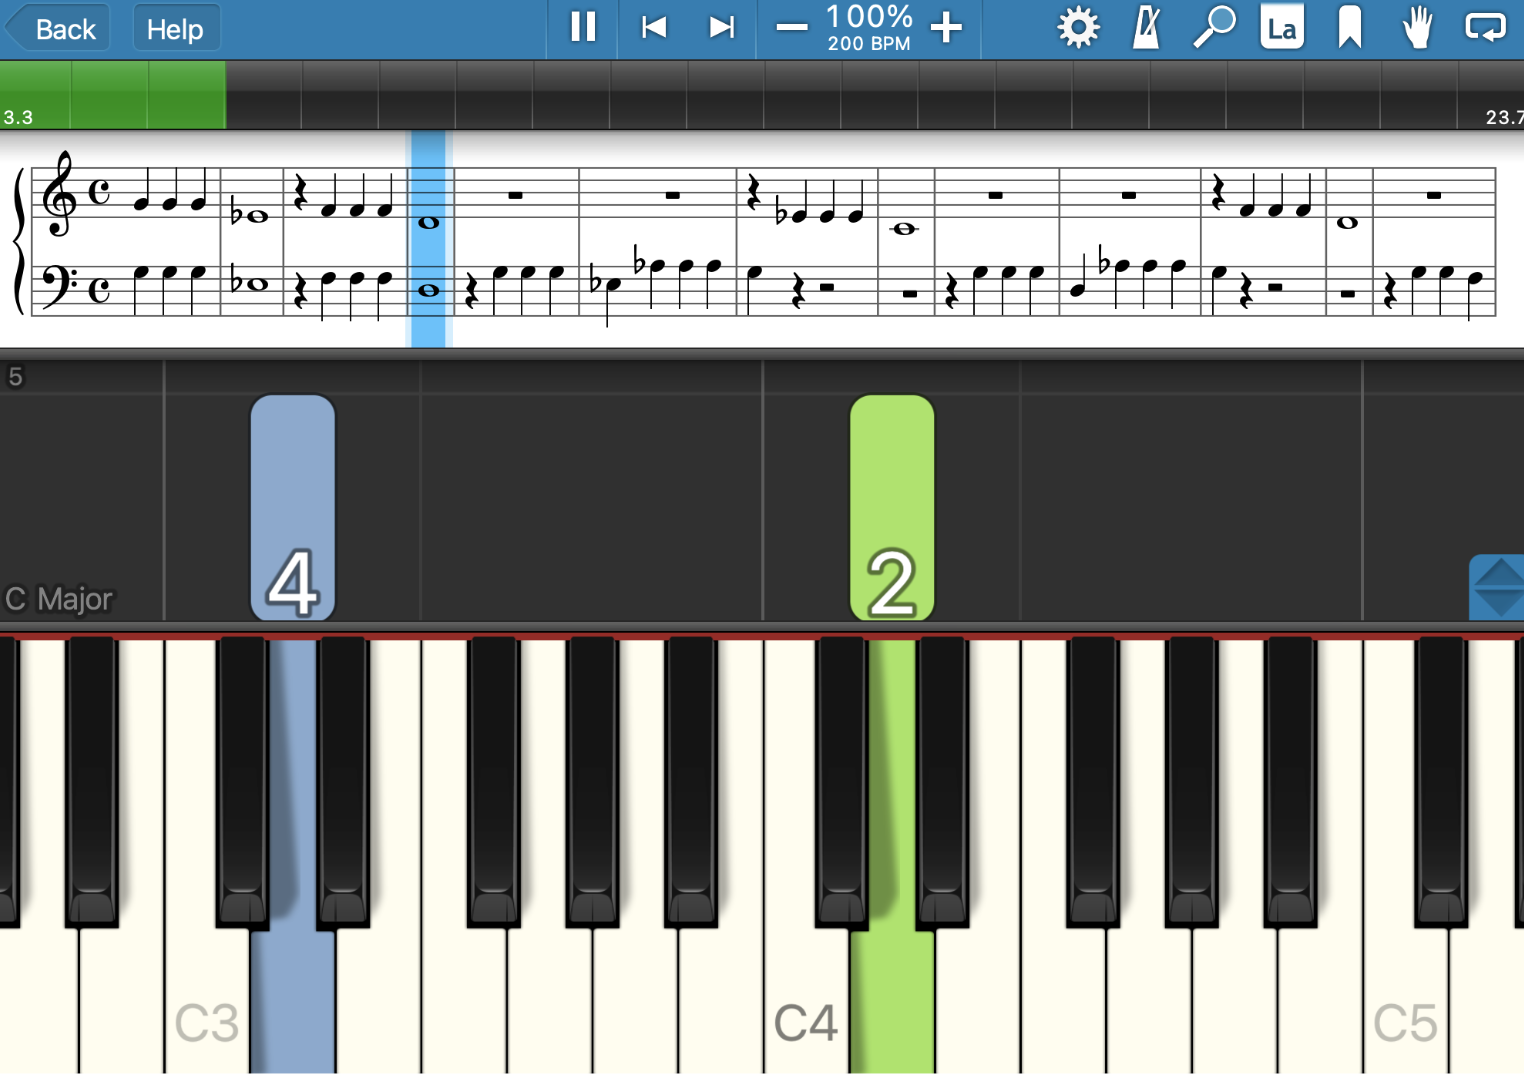
\includegraphics[width=.95\linewidth]{SynthesiaPlaying.png}
    \caption{
       Synthesia attempts to include sheet music and piano roll notation at the same time which results in a cluttered user interface. The size of the piano keys also take up a significant portion of the screen.
    }
    \label{fig:first-page}
\end{figure}


However, the user interface can become very cluttered. When using a smaller MIDI controller, the piano can take up to half of the screen, shortening the time before knowing when to press a note. Additionally, more of the screen is taken up when traditional music notation is on the screen. While the colors and numbers on the notes can be nice, the app receives criticism in the fact that it is not often the correct way to play a piece. The application also introduces a score system, but does not indicate the highest score to strive for besides the number of notes hit versus total number. The prototype design will attempt to fight the cluttered feeling with a smaller piano displayed. The idea of using MIDI files to upload levels will allow for a easy way to get the information of how songs are played and allow the affordance for users to upload their own levels.

\subsection{Rocksmith+}

\textit{Rocksmith+} is a game from Ubisoft's Rocksmith franchise that has been teaching guitar since 2001 and recently dove into teaching piano \cite{RocksmithUbisoft}. The game used the tone set from the game iterations for the guitar with a complete scoring system, particle effects, and a satisfying aesthetic. The game also has lessons worked into the educational aspect to give information about playing the instrument. The user interface effectively communicates which keys users are expected to press by increasing the highlight on the note as the note approaches the keyboard and visually making the digital keys appear pressed down. The one limitation of the game is that users are bound to songs included in the application's library. While a preset category will ensure the correct displayed fingering numbers, users are severely limited in the songs that they are allowed to learn. The preset songs also do not account for users who would like an easier or harder difficulty for the song being played or transposing the song to a different key. Using MIDI files allows users to have this freedom, at the expense of no finger numbers displayed. 


\begin{figure}
    \centering
    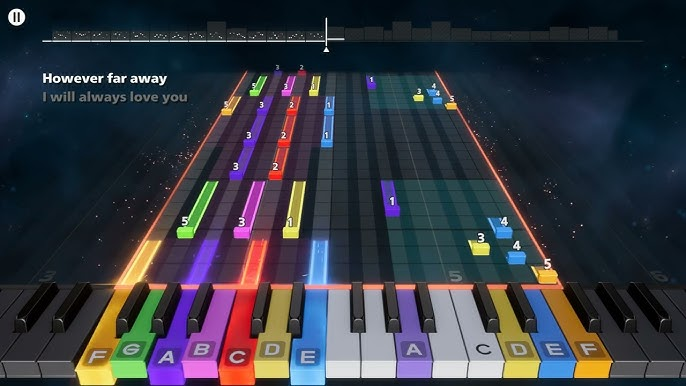
\includegraphics[width=.95\linewidth]{rocksmithpiano.png}
    \caption{
       Rocksmith+ allows people to play the piano to songs in their catalog. Each note is assigned a different color in the piano roll notation.
    }
    \label{fig:first-page}
\end{figure}


\section{Methods and Evaluation}

To begin building the game, much consideration was set for the steps taken to build the game. As discussed above, I will be using the Unity game engine and some packages to include MIDI support in Unity. I installed the software and tested it in an environment to ensure compatibility. 

The game design took the inspiration from \textit{Synthesia} and \textit{Rocksmith+} to create a two-dimensional piano game that uses piano roll notation. The user interface of the prototype was also drafted to follow a rough vision. The initial draft of the user interface included a score in the top left to show users feedback on how they are progressing throughout a song. I also envisioned a digital two-dimensional keyboard on the bottom of the screen that serves the purpose of watching the piano roll notation notes falling onto the notes users are supposed to press. Initially, the falling notes were going to be colored the same with one note prefab similar to \textit{Synthesia}. However, I decided that the notes should be different colors to signify different notes. I hoped that different colors would signify to users the note that they are being asked to press based on the color instead of guessing the horizontal position the note will fall on. 

Core features of the game included the ability to upload MIDI files to allow the user to create song levels. The feature meant that the whole architecture had to revolve around reading and interacting with MIDI files through building levels that spawn the notes at the correct time, knowing when the user has an incorrect input, and interpreting the information sent from the MIDI controller. While I could have created specific levels to my game or make a specific format to my game like \textit{Osu} did with the \textit{.osu} file format, most online music is notated in MIDI, which means it is easily accessible to find or create a song in that format. 

Many of the eventual design choices will be based off of user feedback to determine the most logical way to communicate information to all users. To make progress towards the game, development would be split into two stages. The first stage would be to ensure the basic functionality of a rhythm game. The first playtest would be to primarily receive feedback on the functionality of the game, and design features that users would like to see. The second stage is to receive feedback towards the design choices and how to effectively communicate feedback to the players. 

The nature of the prototype being a game and emphasis on user testing means that majority of the evaluation will be based on how users feel about the game. The participants will be asked to fill out a response form about their experience testing the prototype as well as conducting an interview with me. The questions included in the form will ask about their opinion on potential future features and how to design the game better. Participants will also rate the prototype on a scale of one to ten and if they would play the game again in the future. It is difficult to quantify how respondents 'feel' about their experience, but these questions are a way to understand the state of the prototype and if people had a good enough time to play a game like this in the future. An eventual positive rating and percentage of people that are motivated to play the game again would determine a successful product. The game testing cycle of prototyping, testing, and evaluating means that my methods and evaluation of the project will be tightly knit together. Information that I will be looking for between sessions will be reflected into the included questions of the feedback form. From each testing and evaluation phase, I will determine the next steps for development whether it is revisiting or developing new features to create the best experience for the users. 

The emphasis of the product being a game makes the evaluation focus on the user experience and not if people are correctly learning piano through the prototype. Game testing is more focused on the user interface and user experience while playing a game. If the application was claiming to be a music education tool the methods and evaluation would be completely different. The methods would have to include designing a lesson plan to learn music theory and piano. The lesson plan would attempt to teach the basics and how to advocate for all the teaching problems faced in previous research \cite{PianoTeachingandthePandemic} \cite{E-LearningPiano} \cite{Computer-AssistedInstructionPianoEducation}. Evaluation of a piano education tool would not be able to follow the rapid playtesting cycle to become informed about the effectiveness of the user interface. People do not learn how to play piano over the course of a short test, but would need repeated sessions of playing the game to record score and difficulty improvement. With the constraint of a few months to develop this prototype, evaluating if people are truly learning piano and music would not be possible. 

\subsection{Playtest One}

The core features that would be created and tested for the first playtest is reading the inputted MIDI files for correct note spawn timing, receiving the inputs from the MIDI controller, and making sure that the correct timing of the notes matched the audio. During the process of setting up the foundation of the scene, thoughts of the end goal were kept in mind. I decided that users would play along with an audio file instead of each of their inputs creating a sound. Playing along with an uploaded audio file allows them to know what the song is supposed to sound like while they receive audio signifiers as to whether they are hitting a note correctly or incorrectly. An uploaded audio file also means that uploaded songs that are traditionally heard with a synthesizer, allows users to play along with the synthesizer sound. I also decided to implement a color for each note to communicate the note within the visual octave to the user with the inspiration from Rocksmith+. The colored bar above the keys is to communicate which color is for each key on the piano. 

\begin{figure}
    \centering
    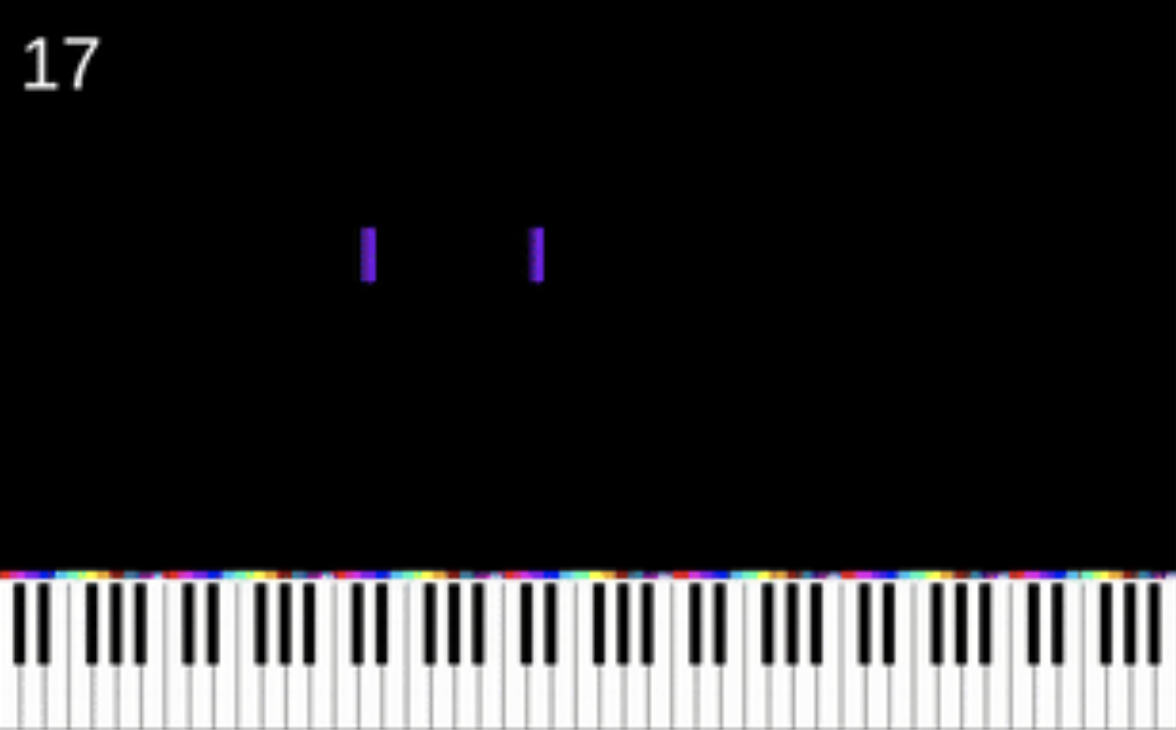
\includegraphics[width=.95\linewidth]{pulsekey-proto0.png}
    \caption{
       Initial prototype with notes in piano roll notation that are a solid color.
    }
    \label{fig:first-page}
\end{figure}

\begin{figure}
    \centering
    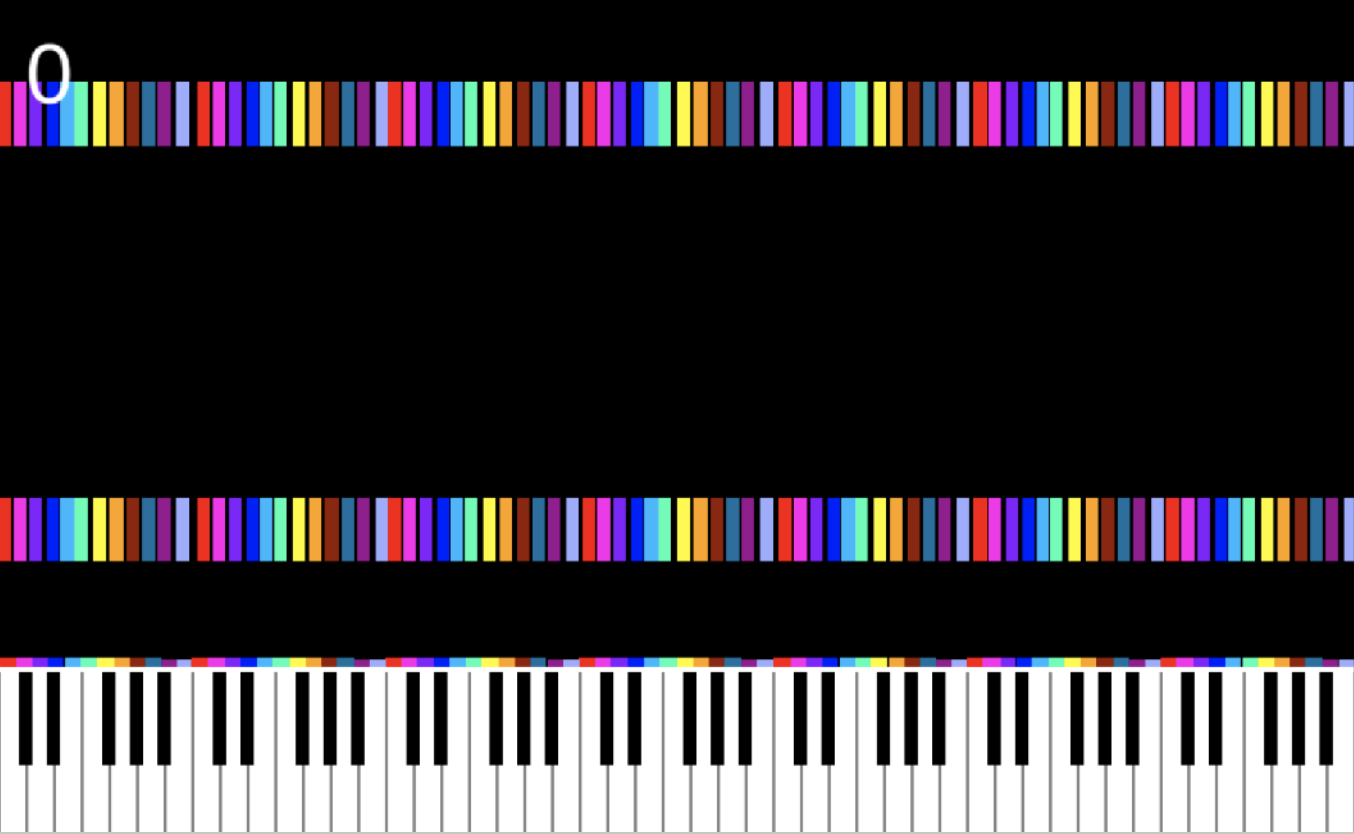
\includegraphics[width=.95\linewidth]{pulsekey-proto1-all notes.png}
    \caption{
       Initial Prototype that demonstrates each note within an octave is a different color and aligns with the color bar on the piano. 
    }
    \label{fig:first-page}
\end{figure}

Before I conducted the first playtest, I tested the initial prototype with a small group to ensure the functionality. Figures 3 and 4 includes a snapshot of the prototype for initial testing. Initial testing demonstrated that the prototype was functional and that the note timing was correct. The participants in the initial testing had no prior experience with piano playing or rhythm games. Participants played a custom song where the notes included are from a C Major chord with limited notes at a time. The limited notes made it so people would not have to move their hands around the piano so they can focus on the timing, but not hindered by the difficulty. Their demographic was useful to help create a low skill floor and know how the information is communicated to users that are unfamiliar in a setting like this prototype. I did receive feedback to include note names on the note and a way to group the notes for an additional way to identify the notes. A participant also asked for the keys on screen to be highlighted when they press a key to know what note they are pressing and orient themselves on the physical keyboard. The feedback given will be incorporated into the official first playtest to observe functionality and receive feedback on the design choices. 


\begin{figure}
    \centering
    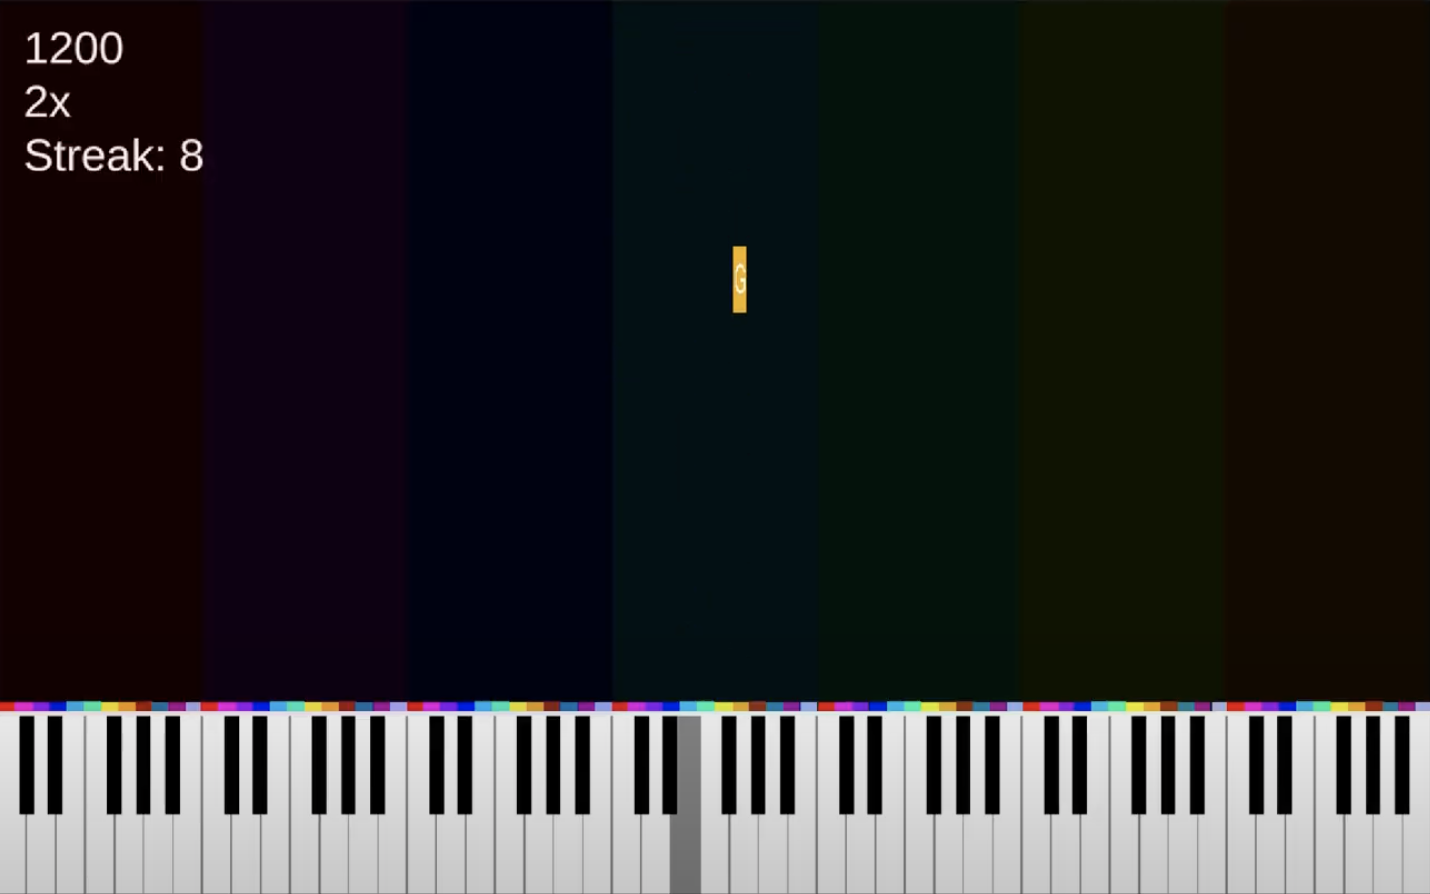
\includegraphics[width=.95\linewidth]{pulsekey-proto-notename.png}
    \caption{
       Prototype as a result from initial informal testing. Added note names on top of falling note, input greys out the key on the digital piano, colored tint for seperated octave, and more scoring information in the interface.
    }
    \label{fig:first-page}
\end{figure}

The first playtest included 10 participants that mostly had no to beginner experience with piano and rhythm games. The participants played the version of the game shown in Figure 5. Participants also played the first song to continue collecting data of the functionality. A summary of the the feedback included having lines separate the octaves instead of colors which would be more defining and people like the black background. Participants also showed interest in a level summary screen so they know the score that they are striving to get. Users suggested different ways to make note information communicated better. Suggestions included making only the keyboard range in the song being included on screen, but they also recognized that it would be weird to see a partial piano on screen. Note names on the keys were suggested, but that would not be meaningful for users that do not piano or music theory because they do not already know the names of the keys. One user suggested to include a line attached to the note to show more specifically where the note would fall on the keyboard. I decided to implement the last suggestion as an experimental feature which could simulate a signifier similar to Rocksmith+ by increasing the highlight of the key for the approaching note.


\subsection{Playtest Two}


The second playtest included the changes listed above shown in Figure 6. The second playtest allowed for users to play the song described earlier for easier difficulty, but also included other levels such as 'Twinkle Twinkle Little Star' for more difficulty. With more functionality and solving problems from the first playtest, allowed for more comments. Players commented to slow down the falling notes so they have more time to process and react. More participants had comments on making the text on the notes more readable. The overall feedback pointed out a variety of bug fixes to create a fluid game experience, but did not point out various new features to incorporate besides slowing down the note speeds. Additionally, users gave feedback about ways to improve replayability and motivation such as a reward system. 


    

\begin{figure}
    \centering
    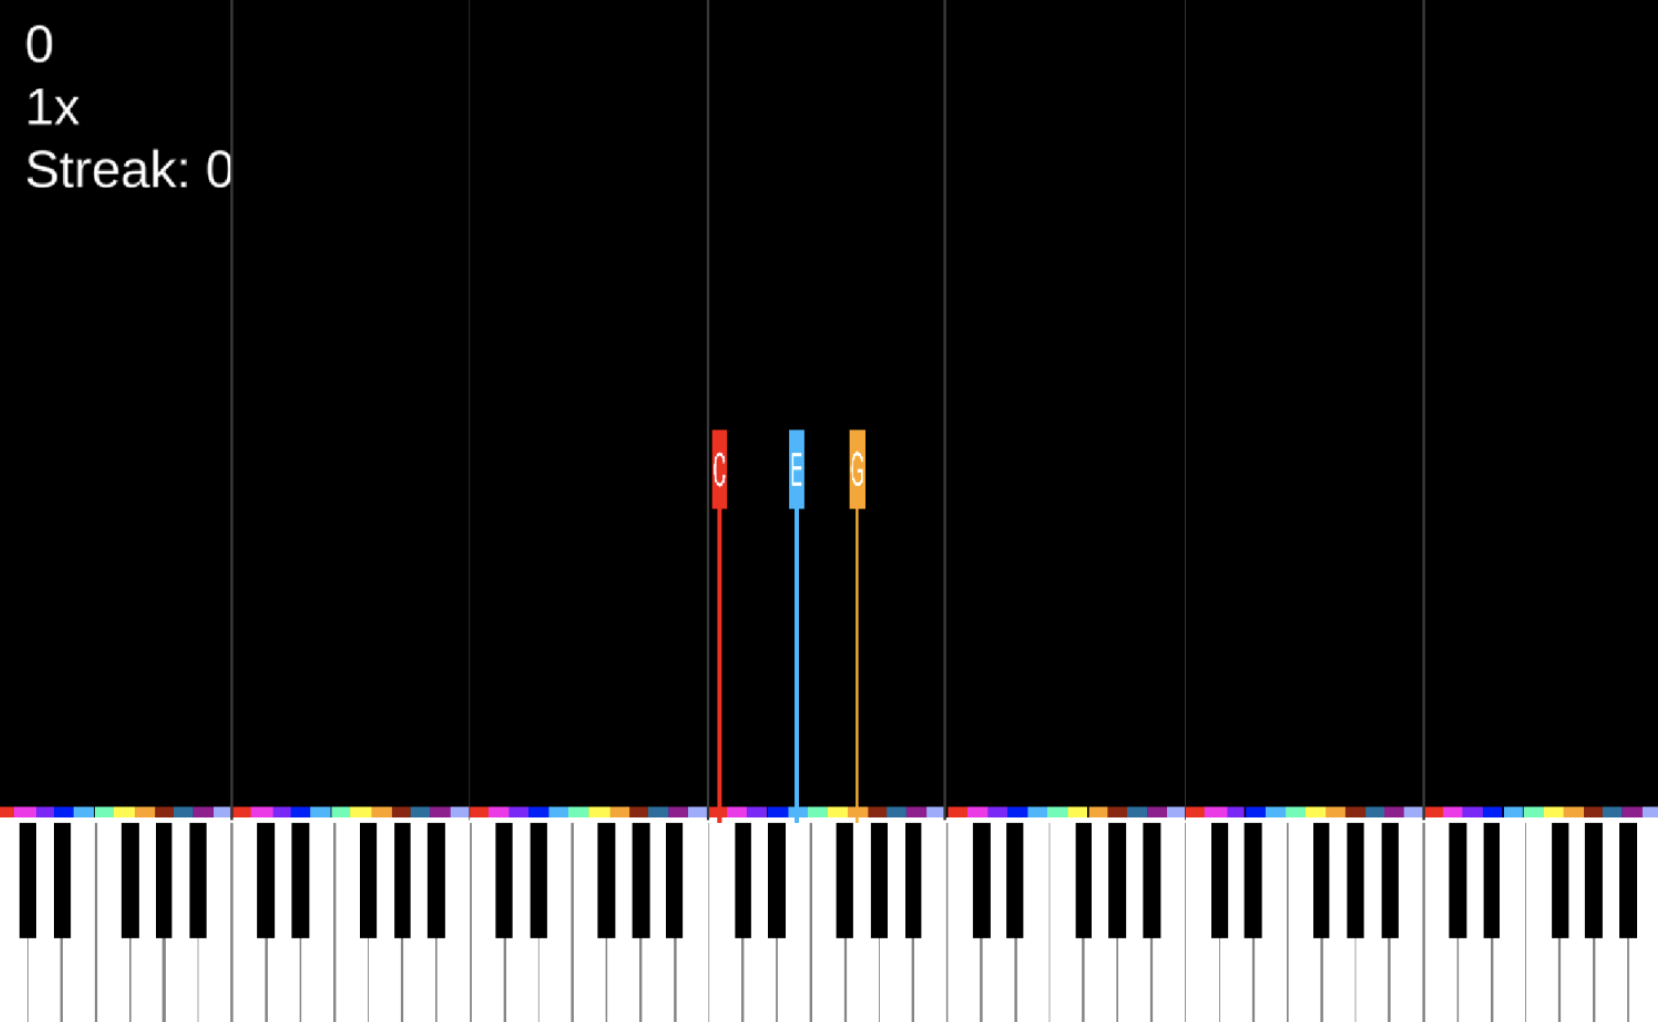
\includegraphics[width=.95\linewidth]{pulsekey-proto2.png}
    \caption{
       Prototype as a result from first playtest. 
    }
    \label{fig:first-page}
\end{figure}

\begin{figure}
    \centering
    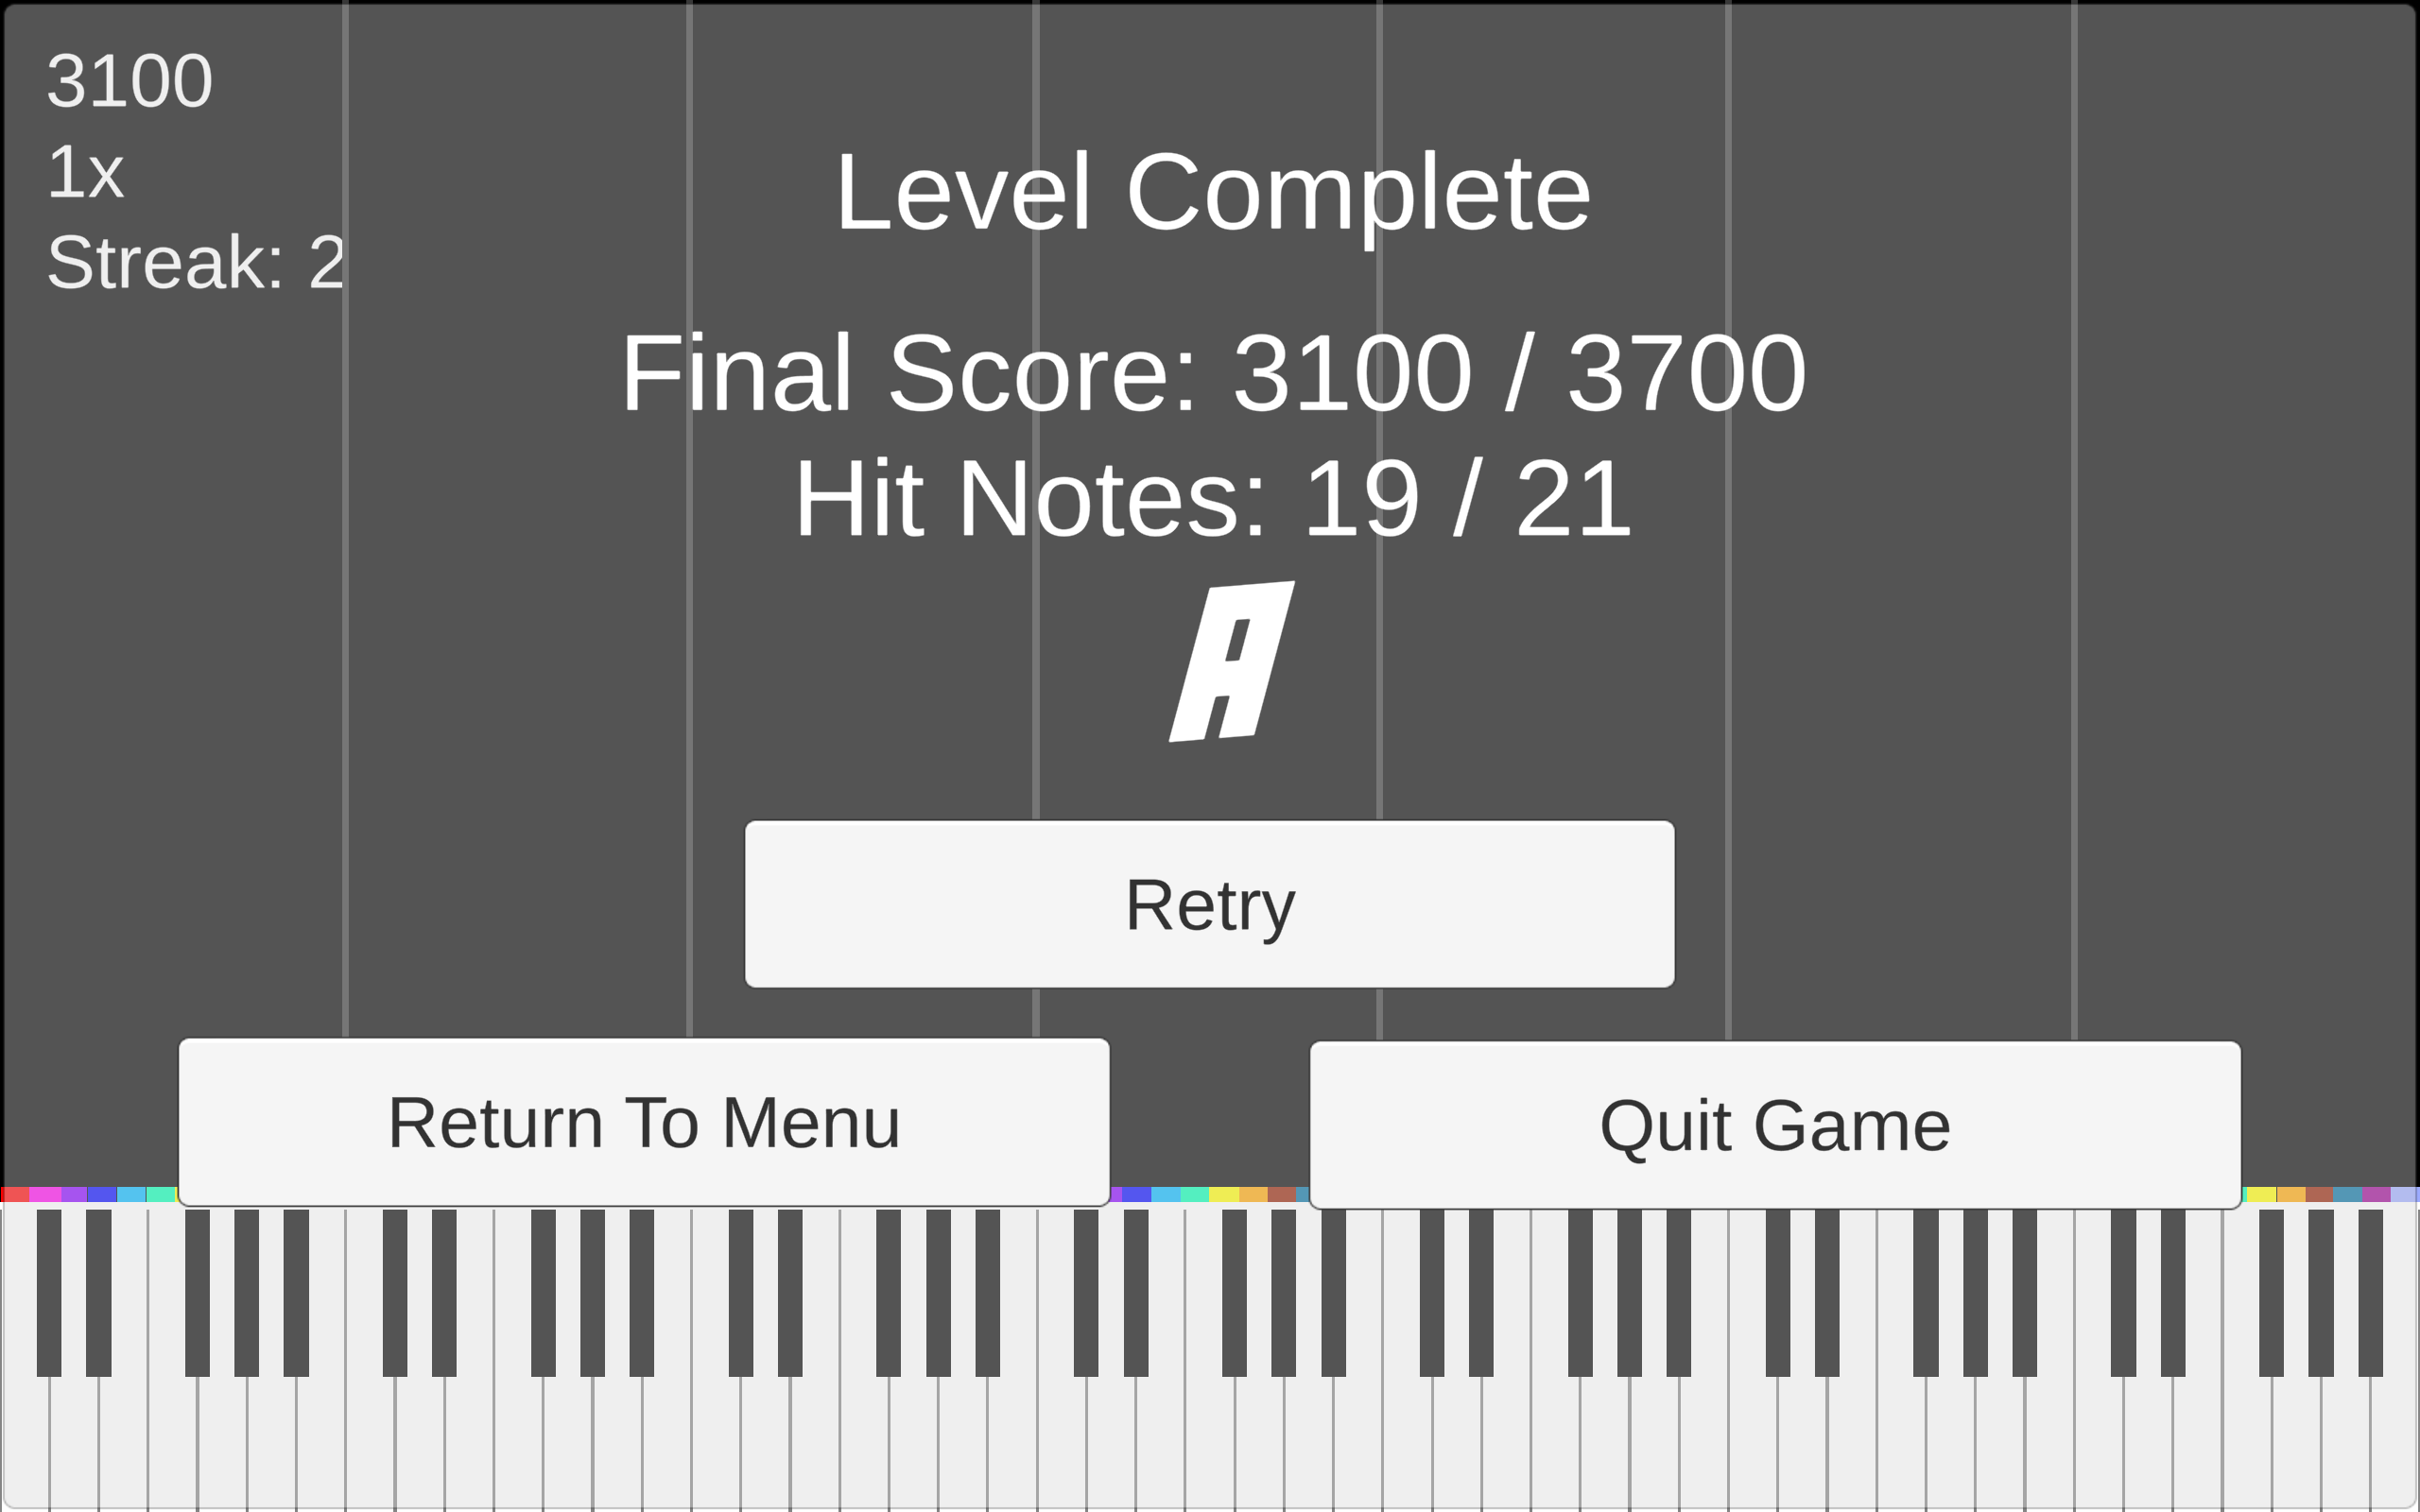
\includegraphics[width=.95\linewidth]{pulsekey-score.png}
    \caption{
       The level summary screen displayed after completing a level. 
    }
    \label{fig:first-page}
\end{figure}

The score summary screen (Figure 7) created at the end of the level resulted in users replaying the levels unprompted signifying a motivation to keep getting a higher score. The score summary screen included the amount of points a play though received out of the maximum number of points, notes hit out of total number of notes, and a letter ranking to indicate their percentage accuracy. The high level of interaction that users had while playing, and willingness to keep playing other songs and trying for higher scores is a reflection of the replayability and motivation to play piano. 

The questionnaire for the second playtest included questions from the Game Experience Questionnaire to learn more about specific experiences created and lacked in my game \cite{GEQpaper}. The questions included from the in-game and post-game modules looked at qualities such as competence, flow, challenge, and more evoked in the user from playing a game \cite{GEQquestions}. 


\section{Results and Discussion}

The prototype succeeded in demonstrating that users would play a game like this again by having 7.75/10 average rating and 75\% of users saying that they would play this game again at the end of playtest two. Contents to the survey responses are included in the repository for this paper. While most research demonstrates that piano education software and current implementations are insufficient at teaching, it is important to remember that people enjoy gamified ways of doing activities and there is a market for that even like playing a piano. Researchers could take these findings to fuel the motivation of incorporating game design into teaching instruments or music education. 

Even though the respondent questionnaires demonstrates a positive review, the Game Experience Questionnaire gives further insight on how to improve the prototype. The in-game question module reveals a fair amount of sensory, moderate positive affect and state of flow, slight sense of competence, and slight to no negative affects. The post-game module reveals slight levels of tiredness and immersion, and slight to moderate levels of positive and negative experience. 

A large number of features need to be incorporated before this prototype can be a competitor to other rhythm games. Respondents stated that note hit animations would not be too distracting to play with. Further testing and design need to be done to figure out a better way to signify which note is falling on which key. The playtests were purposefully conducted on easy levels, but I would need to make sure the current experience lines up with more difficult songs that has more notes. The goal of the game is to have a low skill floor that allows for users that are starting to play piano to understand the information communicated to them, and a high skill ceiling that would allow for a experienced pianist to play any song on the game and have an enjoyable experience. Majority of the demogrpahic in the playtest had no experience with playing piano or with rhythm games which was good for making an accessible game to beginners. 

However, it would also be beneficial to have playtests on a higher skilled pianist and/or rhythm game enthusiast demographic. Higher skilled pianists would have better insight on how to the game feels in comparison to them playing piano. Their comments would be able to describe how it is better or worse from practicing piano on their own. Comments can be addressed to negate negative criticism and also cater to that audience on playing feel. Rhythm game enthusiasts would be able to use their knowledge of other rhythm games to provide user interface comments that can replicate their positive experience from other rhythm games. 

Multiple insights would also be able to assist in the process of raising scores from the game experience questionnaire. Rhythm game enthusiasts would be able to bring suggestions of interactions from other rhythm games to enhance this prototype such as reward systems. Participants suggested including a reward system, but did not specify how, which I believe rhythm game enthusiasts would know how to verbalize. The suggested reward system would be able to raise the positive affect and experience ratings. The questionnaires also reported a moderate negative experience, but did not specify what cause the negative experience in their playthough or if it is an acceptable amount. Players should be penalized for missing notes and incorrect inputs, but the current feedback does not indicate whether the flaw is in the prototype design or the difficulty. 

While I am satisfied with proving that game design will be beneficial in music applications and piano teaching apps that my prototype mimics, I would still do a few steps differently and want to expand the project. Foreseeing the vitality that MIDI files would have in the game was good for the scalability of future levels. However, I did not create full scalability for the user interface of the game. While the levels are created with MIDI and audio files inside the games folders, future development of the game needs to find the functionality to instantiate scenes from the contents inside of a folder which may require reorganization of the directories. 

On a bigger scale I wish I did more research on the options I had to develop my application. While I was able to work in Unity with the installed community libraries, I ran into bugs with the Unity editor such as it having trouble reading my MIDI controller while developing the game. With more time, I would have used Unreal Engine to code the interactions myself. I could have also used a Unity plug-in off of the Unity asset store that is accredited for MIDI support. 

Future development of the game also needs to determine what playerbase to specifically cater for. If experienced piano players demonstrate that they would not play this game, there is no need to have a particularly high skill ceiling. Therefore, the prototype needs more surveying to find the key playerbase and build specifically to the demonstrated interest. I believe that future development and research of the game would reinforce the statistics and findings discussed above.

The evaluation of the prototype was primarily on qualitative aspects by dealing with user interface and user experience. To definitively support my argument, more quantitative reviews would be beneficial. Besides a one to ten rating and the qualities determined by the Game Experience Questionnaire, there are not quantitative aspects. During a in-person presentation, many people played the prototype and gave feedback verbally and was not documented. 

The limited amount of playtesters and limited amount of demographics means there is not a lot of opinions included to understand the general reception of the game. In total there were 14 playtesters across the two playtests. In future work, more playtesters are necessary to deduce the target demographics. Most of the playtesters knew me and could have influenced their responses. I would have liked a better way to grab willing playtesters that did not have any affiliation with me to have completely unbiased results. Some of the playtesters that I knew did not answer the demographic that I thought they would have. Some of the participants had music theory education and took a full year of piano lessons, but still only marked themselves as a beginner piano player. Additionally, some people marked themselves as a beginner without knowing music theory, but followed some song tutorials online and claim to be a beginner. Further surveying would need a more specific way to evaluate users experience with music and piano. Understanding the users experience of music theory, without piano experience, would also be beneficial because they would understand the letters on the notes and the corresponding key on the piano. A similar change would be necessary for evaluating users experience with other rhythm games and what kinds of rhythm games. As discussed previously, some rhythm games emulate instrument playing or dancing while others are clicking circles. Even though both games test rhythm, experience with games that are similar to instruments would be valued as more experience towards games like this prototype. Understanding the players skill level could also influence their reception to this game. In summary, there needs to be a bigger group of playtesters to evaluate the target demographic of the game, and the playtest questionnaire needs to find a better way of evaluating the players skill levels.

\section{Ethical Considerations}
While this game may be made with the best intentions in mind, it still has ethical considerations to take into consideration. 

\subsection{Users with Disabilities}
My game immediately does not account for people who have various disabilities. Whether the disability is visual, auditory, or physical, the game does not have any features to help those users. Not accounting for this group of people, results in cutting out a potential player base. Built-in features for accessibility could be used by players without disabilities to increase player engagement and the quality of their learning experience. 

The application drops the notes from the top of the screen to the bottom onto an area that indicates the moment should press the corresponding key on the physical keyboard. In a paper surveying accessibility in video games, primary stimuli must be perceivable by the player to play a game, and almost all games use visuals as primary stimuli \cite{Yuan}. Additionally, visual impairments can be categorized in terms of blindness, low vision, and color blindness \cite{Bierre}. Primary stimuli are the most important and there are many different types of visual impairments to consider so people can enjoy the game. 

Each note has the note letter attached to the note. The user should be able to change the size of the text for users who wish to make it smaller or larger. For players who are hard of sight, not being able to read the information may hinder their judgement, leading to frustration. Players who are not hard of sight may also enjoy these features to either make the visual cues easier to read or make them smaller if they are too distracting. 

Additionally, the text and notes are colored so there needs to be an option for the users to change the color that appears for the visual cues. Allowing the option for the user to change the color of the text will allow the user to focus on the color of the visual cue to know how they are doing while playing the song. The option to manually set the color for each attribute would be ideal so the application can cater to user-specific visual needs. A color associated with each note allows the user to associate each note with a color without having to strain their vision to guess where the note may line up. However, the default color scheme set in the prototype may be nonsensical to some of the playtesters. User options to set the colors and overall color scheme will help communicate the information to the player based on their individual needs. These accessibility options for manually setting the colors for each attribute will also be beneficial for users without visual impairments to customize their specific set-up.


There are many reasons for a user to have a physical disability while playing the game. “Motor-impaired players are limited in their ability to provide input physically” \cite{Yuan}. Physical limitations could range from permanent disabilities such as not having a finger to temporary mobility loss like a sprained finger resulting in the player not being able to physically input what they cognitively know they have to do \cite{Bierre}. 
 
A player knowing what they have to do, physically not able to do the action, and being deducted score-wise would be very frustrating. An argument would be to only upload MIDI files that they can play, or for them to alter the MIDI file to fit their own needs. However, this shoves all the faults onto the player instead of adding some functionality within the application to assist the user. There are many options to fix this. One way would be to add a feature that lets the player choose which notes should not count before playing the track. For example, if a user is physically unable to stretch their hands an octave, allow them to only hit one of the notes in the octave.

An additional solution would be to add the option to slow down the song by a percentage to give a little extra time to those who need it. “Where a gamer has slow reaction times, games can be rendered impossible without a speed control or wide difficulty level adjustment” \cite{Bierre}. These accessibility options would indirectly benefit abled users because they would be able to learn in stages to learn the full song. People with slow reaction times are not the only people to benefit, people that physically can not move fast enough would benefit from this feature. 

\subsection{Replacing Traditional Music Lessons}

The application is marketed as a game and not as educational software, but how closely it resembles gameplay from other applications that claim to teach piano, it is easy to see how people would attempt to use the application as a replacement to learn piano. Even though my paper critiques other applications, they still teach ideas and concepts, but are unable to reinforce them in students. A core issue of being unable to reinforce musical performance concepts is that people will not learn techniques and phrasing to play the song as it heard. People will then be unable to replicate what they think they sound like leaving them in a frustrated state with reinforced bad habits. 

\begin{figure}
    \centering
    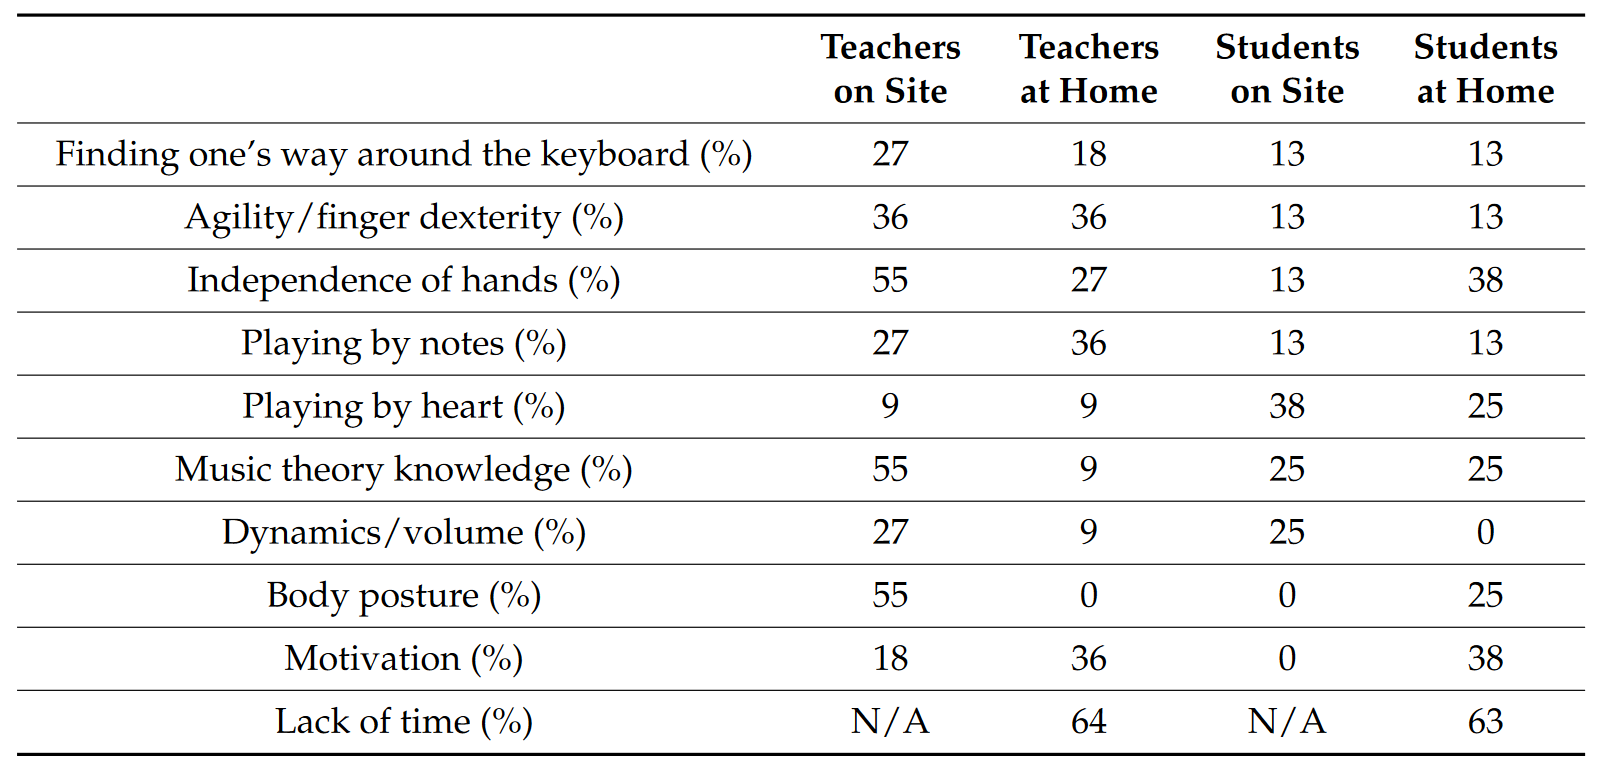
\includegraphics[width=.95\linewidth]{PianoLearningProblemsTable.png}
    \caption{
       Reported problems during piano lessons and during independent home practice \cite{PianoTeachingAndLearningConcerns}. Teachers’ and students’ responses presented as percentages. Multiple responses were possible.
    }
    \label{fig:first-page}
\end{figure}

Similar studies have attempted to understand the impact software applications have on teaching music. Figure 8 shows a survey of some of the problems that teachers and students had with a piano software application \cite{PianoTeachingAndLearningConcerns}. Students between on-site lessons and at home have relatively similar concerns when learning the piano. However, the increased concerns for on-site can be because students are made aware by their teachers. Additionally, teachers' increased concerns while on-site, can be a direct translation of them making the students aware of issues at the moment. The application will only be able to tell the student about whether they are on time and if they hit the correct note. Therefore, students who do not know the mistakes they are making in other aspects such as posture and hand position, in the way they are notified by a teacher, would build up bad habits because the game is rewarding what they are doing, or get frustrated because they do not know why they are not able to play the song. 

Additionally, using this software to substitute music education will reduce the amount of people that wish to learn from instructors and music teachers. Sources such as instructors and music teachers share most of the information that is needed to play a piece with the correct technique. An application, especially this prototype, is one-dimensional in the sense that a note being pressed is either right or wrong. Performance practice in music refers to the study and application of the techniques, styles, conventions, and interpretative approaches that are historically or culturally appropriate to the performance of music from a particular time period, geographical region, or genre. Only learning from an application means that people will not be informed of the extra information beyond the notes. Performances also include the performer incorporating their own individualistic touch on the notes to make it their own. If music was taught in a one-dimensional sense without performance practice and individualism, there would be no purpose to play music on your own or listen to specific performers over a recording. Therefore, instructors and music teachers are vital to preserving the art of music.

\printbibliography

\appendix
\appendixpage
\addappheadtotoc
\section{Replication Instructions}

To clone my project, you must have Unity installed on your computer. If you do not have Unity or the Unity hub installed, go to unity.com/download to download Unity hub for your computer's operating system. Open up the installer, agree to the terms, select your destination folder, and select install. Once installed, open up the Unity Hub application. The application will prompt you to download the latest Unity Editor. You are welcome to do so, but the prototype was created in version 2021.3.38f1. To do so, locate the installs panel on the side, and click the intall editior button. If the version is not listed, go to archive and press download archive which will open a page. Navigate to version 2021.3.38f1, click install, and you will be brought back to Unity hub to select modules. Make sure that Microsoft Visual Studio Community 2022 and build support for your operating system. If you are prompted about not having a license, create a unity account with your desired license and log in your account in Unity Hub. 

Once Unity Hub and the correct Unity version is installed, you are ready to download the project from Git Hub. Click on the green code button and download the zip file. After downloading the zip file, extract the contents of the zip file. Go back to Unity Hub and the Projects tab. Click the add button and "add project from disk." After selecting the location of the extracted zip folder, the folder name should show up in the projects list. Click on the project with the correct editor version to open up the project. Navigate to the scenes to open up a level and play. The prototype was developed in the 16:10 aspect ratio. 

All the packages and github plug-ins are included in the project. However, the versions of the packages used in the project are listed below in Figure 9. Links to the github installs of DryWetMIDI, Minis, and MidiJack can be found in the references if there are any issues when opening the project \cite{drywetmidi}\cite{minis}\cite{midijack}.


\begin{figure}[h]
    \centering
    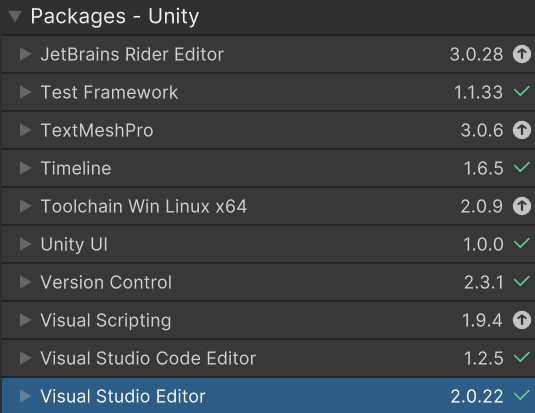
\includegraphics[width=.95\linewidth]{UnityPackages.png}
    \caption{
       The packages and versions used in the Unity project
    }
    \label{fig:first-page}
\end{figure}


\section{Code Architecture Overview}
On the start of a song, the SongManager gameobject has an instance of the SongManager scrip that includes a reference to an AudioSource object, the file location of the MIDI file, and an array of Lanes that includes a reference to each lane in the editor. The SongManager script interprets the MIDI file and sends the note time stamps to the individual lanes, and starts the audio source. The Keyboard script generates the digital keyboard visualizer from the WhiteTile and BlackTile gameobjects.

\begin{figure}
    \centering
    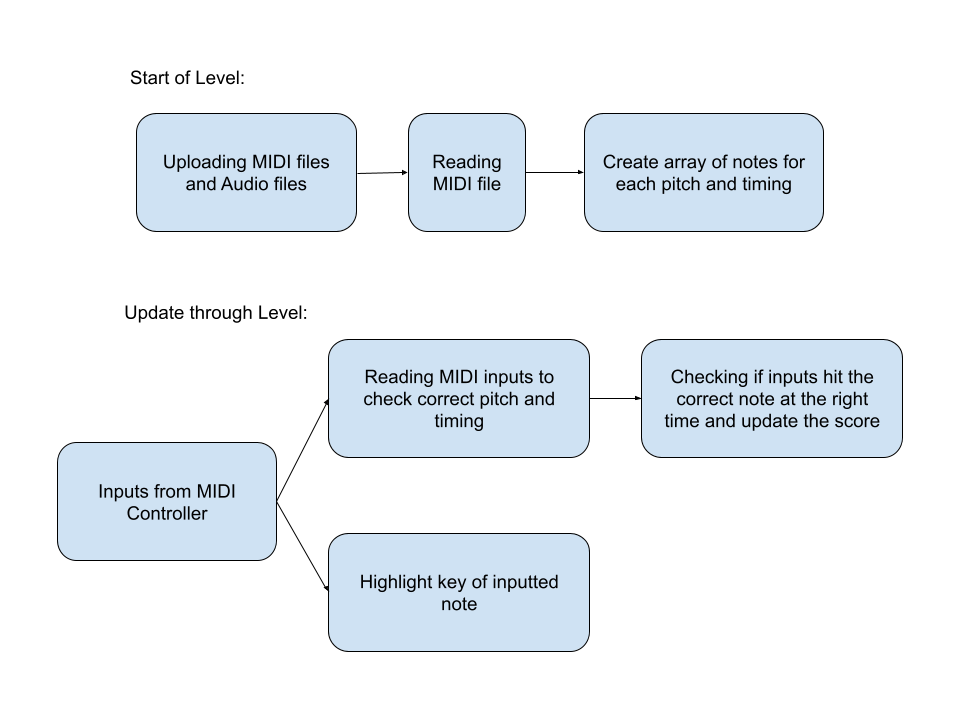
\includegraphics[width=.95\linewidth]{CS Comps Architecture.png}
    \caption{
       Overview of Pulsekey prototype architecture 
    }
    \label{fig:first-page}
\end{figure}

During the song, multiple parts move at once. Each Lane object has a lane script that spawns a note at the specified time stamp given by the SongManager for visualization. The lane script checks the MIDI input against the array to determine if the note was hit correctly which passes the information to the ScoreManager. The ScoreManager listens for the Lanes to communicate if a note was hit or missed, then updates the score accordingly. The Pianotile script is attached to the WhiteTile and BlackTile gameobjects to listen for the MIDI inputs and switches between the start color of the object and gray. The SongManger also includes the PauseMenu script with references to the PauseMenu canvas overlay and audio to pause the level.

The score manager checks if the song was completed then pops up a level complete screen that displays the score information from within the script. The overlay also consists of buttons from the PauseMenu script to retry the level, return to the menu, and quit the application.



\end{document}
